% Created 2015-09-07 Mon 19:24
\documentclass[11pt]{article}
\usepackage[utf8]{inputenc}
\usepackage[T1]{fontenc}
\usepackage{fixltx2e}
\usepackage{graphicx}
\usepackage{longtable}
\usepackage{float}
\usepackage{wrapfig}
\usepackage{rotating}
\usepackage[normalem]{ulem}
\usepackage{amsmath}
\usepackage{textcomp}
\usepackage{marvosym}
\usepackage{wasysym}
\usepackage{amssymb}
\usepackage{capt-of}
\usepackage{hyperref}
\tolerance=1000
\usepackage[utf8]{inputenc}
\usepackage{commath}
\usepackage{pgf}
\usepackage{tikz}
\usetikzlibrary{shapes,backgrounds}
\usepackage{marginnote}
\usepackage{listings}
\usepackage{enumerate}
\usepackage{algpseudocode}
\usepackage{algorithm}
\usepackage{mathtools}
\usetikzlibrary{arrows,automata}
\setlength{\parskip}{16pt plus 2pt minus 2pt}
\renewcommand{\arraystretch}{1.6}
\DeclareMathOperator{\Neg}{Neg}
\author{Oleg Sivokon}
\date{\textit{<2015-09-04 Fri>}}
\title{Assignment 11, Authomata Theory}
\hypersetup{
 pdfauthor={Oleg Sivokon},
 pdftitle={Assignment 11, Authomata Theory},
 pdfkeywords={Automata Theory, Formal Languages, Assignment},
 pdfsubject={First assignment in the course 20440 Automata and Formal Languages},
 pdfcreator={Emacs 25.0.50.1 (Org mode 8.3beta)}, 
 pdflang={English}}
\begin{document}

\maketitle
\tableofcontents

\definecolor{codebg}{rgb}{0.96,0.99,0.8}
\definecolor{codestr}{rgb}{0.46,0.09,0.2}
\lstset{%
  backgroundcolor=\color{codebg},
  basicstyle=\ttfamily\scriptsize,
  breakatwhitespace=false,
  breaklines=false,
  captionpos=b,
  framexleftmargin=10pt,
  xleftmargin=10pt,
  framerule=0pt,
  frame=tb,
  keepspaces=true,
  keywordstyle=\color{blue},
  showspaces=false,
  showstringspaces=false,
  showtabs=false,
  stringstyle=\color{codestr},
  tabsize=2
}
\lstnewenvironment{maxima}{%
  \lstset{%
    backgroundcolor=\color{codebg},
    escapeinside={(*@}{@*)},
    aboveskip=20pt,
    captionpos=b,
    label=,
    caption=,
    showstringspaces=false,
    frame=single,
    framerule=0pt,
    basicstyle=\ttfamily\scriptsize,
    columns=fixed}}{}
}
\makeatletter
\newcommand{\verbatimfont}[1]{\renewcommand{\verbatim@font}{\ttfamily#1}}
\makeatother
\verbatimfont{\small}%
\clearpage

\section{Problems}
\label{sec:orgheadline19}

\subsection{Problem 1}
\label{sec:orgheadline3}
Given following languages over the alphabet \(\{a, b\}\)
\begin{itemize}
\item \(L_1 = \emptyset\).
\item \(L_2 = \{\epsilon, aa\}\).
\item \(L_3 = \{\epsilon, a, aa, ab, abb\}\).
\item \(L_4 = \{aabb, aabbb, aa, aaa\}\).
\item \(L_5 = \{\epsilon, b, bbb, abab, abba, aabb\}\).
\item \(L_6 = \{\epsilon, bbbaa, baba, aaab, aabba, aa\}\).
\end{itemize}


\begin{enumerate}
\item What are the following languages:
\begin{itemize}
\item \(L_4L_4\).
\item \((L_1 \cup L_2 \cup L_3)^R\).
\item \(L_3L_1L_6\).
\end{itemize}

\item Define exponentiation as follows:
\(L^K = \{x \in L \;|\; \exists y \in K.(\abs{y} = \abs{x})\}\).
What are the languages \(L_4^{L_5}\) and \(L_6^{L_1}\)?
\end{enumerate}

\subsubsection{Answer 1}
\label{sec:orgheadline1}
\begin{enumerate}
\item Concatenation of \(L_4\) with itself gives:
\(L_4L_4 = \{aabbaabb, aabbaabbb, aabbaa,\;\) \(aabbaaa, aabbbaabb,
       aabbbaa, aabbbaaa, aaaabbb, aaaa, aaaaa, aaaaabb, aaaaabbb\}\)
\item \((L_1 \cup L_2 \cup L_3)^R = \{\epsilon, a, aa, ba, bba\}\).
\item \(L_3L_1L_6 = \emptyset\).  This is so because there are no words
in language \(L_1\) to concatenate with.
\end{enumerate}


\lstset{language=prolog,label= ,caption= ,captionpos=b,numbers=none}
\begin{lstlisting}
:- use_module(library(lists)).

concatentated_member(L1, L2, L3) :-
    member(M1, L1), member(M2, L2),
    string_concat(M1, M2, L3).

concatentated(L1, L2, L3) :-
    findall(X, concatentated_member(L1, L2, X), X),
    list_to_set(X, L3).

assignment_11a :-
    X = ["aabb", "aabbb", "aa", "aaa"],
    concatentated(X, X, Y),
    [First | Rest] = Y,
    write("$$\\{"),
    write(First),
    maplist(format(',\\allowbreak ~s'), Rest),
    write("\\}$$").
\end{lstlisting}

\(\{aabbaabb,\allowbreak aabbaabbb,\allowbreak aabbaa,\allowbreak aabbaaa,\allowbreak aabbbaabb,\allowbreak aabbbaabbb,\allowbreak aabbbaa,\allowbreak aabbbaaa,\allowbreak aaaabb,\allowbreak aaaabbb,\allowbreak aaaa,\allowbreak aaaaa,\allowbreak aaaaabb,\allowbreak aaaaabbb,\allowbreak aaaaaa\}\)

\subsubsection{Answer 2}
\label{sec:orgheadline2}
\begin{enumerate}
\item \(L_4^{L_5} = \{aaa, aabb\}\).
\item \(L_6^{L_1} = \emptyset\).
\end{enumerate}

\subsection{Problem 2}
\label{sec:orgheadline6}
Let \(L_1, L_2\) and \(L_3\) be languages over some alphabet \(\Sigma\).
Prove or disprove:
\begin{enumerate}
\item \((L_1 \cup L_2) L_3 = L_1 L_3 \cup L_2 L_3\).
\item \((L_1 \cap L_2) L_3 = L_1 L_3 \cap L_2 L_3\).
\end{enumerate}

\subsubsection{Answer 3}
\label{sec:orgheadline4}
First, I will prove \((L_1 \cup L_2) L_3 \subset L_1 L_3 \cup L_2 L_3\).
Assume to the contrary that there is \(w \in (L_1 \cup L_2) L_3\) which is not
in \(L_1 L_3 \cup L_2 L_3\).  Put \(w = xy\) where \(x \in (L_1 \cup L_2)\) and \(y
    \in L_3\) (this implies \(L_3 \neq \emptyset\) and at least one of \((L_1 \cup
    L_2) \neq \emptyset\).  Suppose \(x\) comes from \(L_1\), then it has to be in
\(L_1 L_3 \cup L_2 L_3\) because it is in L\(_{\text{1}}\) L\(_{\text{3}}\)\$, similartly if it originates
in \(L_2\).  Suppose now \(L_3 = \emptyset\), then there is an empty set on
both sides of equation (by definition of concatenation).  Suppose both \(L_1\)
and \(L_2\) are empty, then, again, we have emtpy set on both sides of the
equation.  Thus we showed that it is impossible for \(w\) not to be in the
\(L_1 L_3 \cup L_2 L_3\), hence the original argument must be true.

Similarly, to prove \(L_1 L_3 \cup L_2 L_3 \subset (L_1 \cup L_2) L_3\),
assume there exists \(w \in L_1 L_3 \cup L_2 L_3\), not a amember of \((L_1
    \cup L_2) L_3\).  Again, \(w = xy\) where \(y \in L_3\) and \(x\) may be a
member of \(L_1\), \(L_2\) or both.  Suppose, again, the sets aren't empty.
If \(w\) came from \(L_1 L_3\), then \(x\) came from \(L_1\), but it is a member
of \((L_1 \cup L_2)\) and similarly if it came from \(L_2\).  Since \(y \in L_3\)
and \(L_3\) is present on both sides, it is not possible for \(w\) to not
be a member of \((L_1 \cup L_2) L_3\).  As in previous case, whenever \(L_3\)
or \((L_1 \cup L_2)\) are empty, both sides of equation contain an empty set.
Hence we proved both directions, hence the conjecture is true.

\subsubsection{Answer 4}
\label{sec:orgheadline5}
This conjecture isn't generally true.  Suppose \(L_1 = L_3 = \{a\}\) and
\(L_3 = \{\epsilon, aa\}\).  Then:

\begin{enumerate}
\item \((L_1 \cap L_2) L_3 = \emptyset\).
\item \(L_1 L_3 \cap L_2 L_3 = \{aa\}\).
\end{enumerate}

I.e. both sides of equation are not equal.  This completes the proof.

\subsection{Problem 3}
\label{sec:orgheadline9}
An equivalence relation over \(\Sigma^*\) will be called invariant from
right if \(\forall z \in \Sigma^*.(xRy \implies xzRyz)\).  Answer for
every relation in \(\{a, b\}^*\) whether the relation is an equivalence
relation and whether it is invariant from right.

\begin{enumerate}
\item \(xRy \iff \abs{x} \geq \abs{y}\).
\item \(xRy \iff (\abs{x} = \abs{y} = 0 \lor x = qz, y = pz, \abs{z} \geq 1)\).
\end{enumerate}

\subsubsection{Answer 5}
\label{sec:orgheadline7}
Total order relation is not symmetric.  Suppose \(x = a\) and \(y = ab\), then
\(x \geq y\) but not \(y \geq x\).  Since this relation is not an equivalence,
it cannot be right invariant either.

\subsubsection{Answer 6}
\label{sec:orgheadline8}
This relation is an equivalence.  It is transitive because whenever
\(x = qz\), \(y = pz\) and \(w = vz\), all of the below hold: \(xRy\), \(yRw\),
\(xRw\) since they all have the last letter in common.  This also holds
trivially in case the length is zero, since \(x = y = w = \epsilon\) in
that case.

The relation is reflexive because whenever every string is either
empty or its last symbol is equal to itself, i.e. \(xRx\) is always true.

The relation is symmetric because whenever \(x = qz\) and \(y = pz\) then
both \(xRy\) and \(yRx\) hold (again, becuase \(x\) and \(y\) have the final
letter in common, or are both the empty string).

The relation is also invariant from the right.  The proof will proceed
by induction on the string's length.

\textbf{Base step:} \(\epsilon R \epsilon \implies \epsilon z R \epsilon z\) because
\(R\) is reflexive and \(z = \epsilon z\).

\textbf{Inductive step:} suppose the inductive hypotesis \(xRy \implies xzRyz\), then
suppose we concatenate the same character \(c\) to both \(x\) and \(y\).  This
character must be the same by definition of \(R\).  Then \(xcRyc \implies
    xczRycz\) because we can simply rename \(xc = x_1\) adn \(yc = y_1\) and obtain
the inductive hypothesis restated using new terms: \(x_1Ry_1 \implies
    x_1zRy_1z\).  This completes the inductive step, and hence the proof is
completed.

\subsection{Problem 4}
\label{sec:orgheadline12}
Build an DFA accepting languages over alphabet \(\{a, b\}\) s.t.
\begin{enumerate}
\item The language contains all words with a substring \(abb\), but never
with the substring \(aa\).
\item If the word contains substring \(bb\) must, it must be preceded by \(aba\).
\end{enumerate}

\subsubsection{Answer 7}
\label{sec:orgheadline10}
Below is the DFA for the first question:

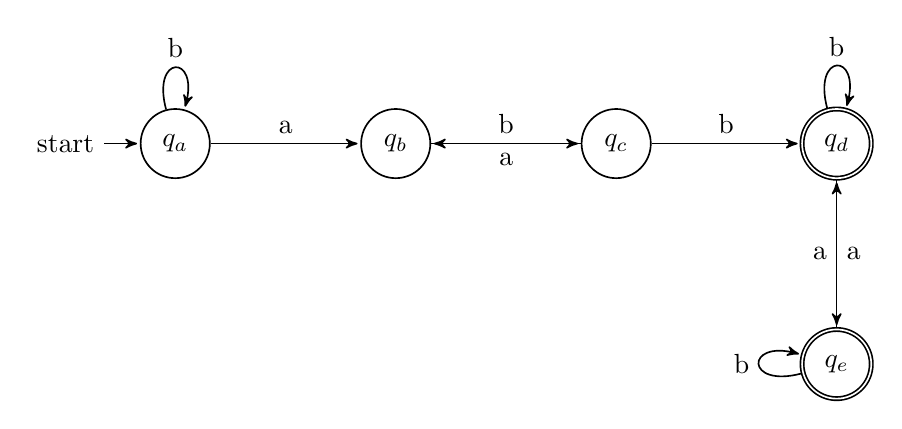
\begin{tikzpicture}[->,>=stealth',shorten >=1pt,auto,node distance=2.8cm,
                    semithick]

  \node[initial,state]    (A)              {$q_a$};
  \node[state]            (B) [right of=A] {$q_b$};
  \node[state]            (C) [right of=B] {$q_c$};
  \node[accepting,state]  (D) [right of=C] {$q_d$};
  \node[accepting,state]  (E) [below of=D] {$q_e$};

  \path (A) edge [loop above] node {b}   (A)
            edge              node {a}   (B)
        (B) edge              node {b}   (C)
        (C) edge              node {a}   (B)
            edge              node {b}   (D)
        (D) edge [loop above] node {b}   (D)
            edge              node {a}   (E)
        (E) edge [loop left]  node {b}   (E)
            edge              node {a}   (D);
\end{tikzpicture}


\emph{Nodes where the automata dies are not shown.}

\subsubsection{Answer 8}
\label{sec:orgheadline11}
Below is the DFA for the second question:

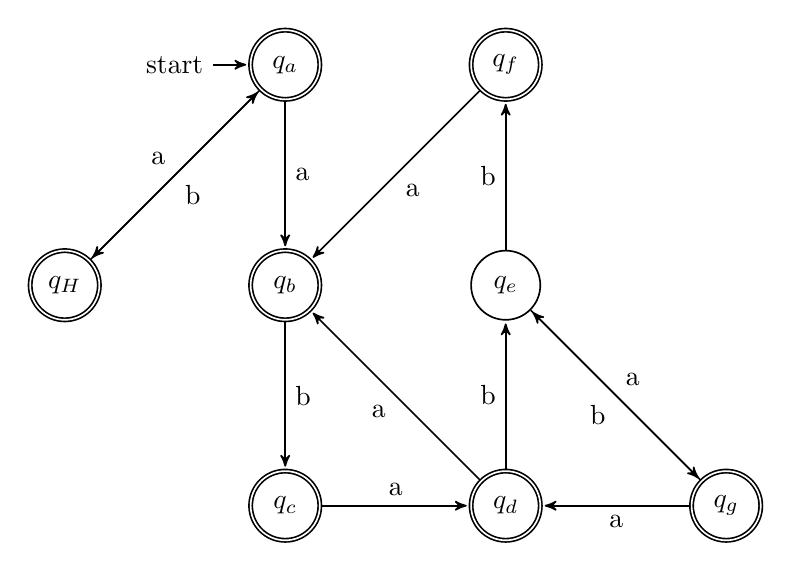
\begin{tikzpicture}[->,>=stealth',shorten >=1pt,auto,node distance=2.8cm,
                    semithick]

  \node[accepting,initial,state] (A)              {$q_a$};
  \node[accepting,state]         (B) [below of=A] {$q_b$};
  \node[accepting,state]         (C) [below of=B] {$q_c$};
  \node[accepting,state]         (D) [right of=C] {$q_d$};
  \node[state]                   (E) [above of=D] {$q_e$};
  \node[accepting,state]         (F) [above of=E] {$q_f$};
  \node[accepting,state]         (G) [right of=D] {$q_g$};
  \node[accepting,state]         (H) [left of=B]  {$q_H$};

  \path (A) edge node {a} (B)
            edge node {b} (H)
        (B) edge node {b} (C)
        (C) edge node {a} (D)
        (D) edge node {b} (E)
            edge node {a} (B)
        (E) edge node {b} (F)
            edge node {a} (G)
        (F) edge node {a} (B)
        (G) edge node {a} (D)
            edge node {b} (E)
        (H) edge node {a} (A);
\end{tikzpicture}


\emph{Nodes where the automata dies are not shown.}

\subsection{Problem 5}
\label{sec:orgheadline15}
Given alphabet of binary strings and netation operation defined as
follows:
\begin{align*}
  \Neg(w) = \begin{cases}
    \epsilon  &\mbox{if } w = \epsilon \\
    1         &\mbox{if } w = 0 \\
    0         &\mbox{if } w = 1 \\
    0.\Neg(y) &\mbox{if } w = ay \land a = 1 \\
    1.\Neg(y) &\mbox{if } w = ay \land a = 0\;.
  \end{cases}
\end{align*}

And similarly for languages: \(\Neg(L) = \{w \;|\; \Neg(w) \in L\}\).

\begin{enumerate}
\item Does there exist a language \(\overline{L} = \Neg(L)\)?
\item Does there exist a language \(\overline{L} \setminus \{\epsilon\} = \Neg(L)\)?
\end{enumerate}

\subsubsection{Answer 9}
\label{sec:orgheadline13}
No, there cannot be such language.  Suppose there was such a language, then
\(\epsilon\) must be either in it or in its complement.  Suppose \(\epsilon\) is
part of \(L\), then it must be also in its negation since \(\epsilon =
    \Neg(\epsilon)\).  By symmetric reasoning \(\epsilon\) cannot be in \(\overline{L}\).

\subsubsection{Answer 10}
\label{sec:orgheadline14}
Yes, there exists such a language, for instance the language representing all
odd numbers in base 2.  Its complement would be a language representing all
even numbers in base 2 and because words in \(L\) always end in 1 (with no other
requirements) negating them will necessarily produce a word in \(\overline{L}\).

No number is both odd and even, therefore negation produces exactly the
complement of \(L\).  Since empty string is excluded, the only word which would
be also a negation of itself is excluded as well.

\subsection{Problem 6}
\label{sec:orgheadline18}
\begin{enumerate}
\item Given DFAs \(A = (\Sigma, Q, q_0, F, \delta)\) and \(B = (\Sigma, Q, q_0, F
      \cap (Q \setminus q_0), \delta)\), is it also the case that \(L(B) = L(A)
      \cap \Sigma^+\)?
\item Given DFA \(A = (\Sigma, Q, q_0, F, \delta)\) construct DFA \(B\) from \(A\)
s.t. it accepts all words of the language of \(A\) which have length
distinct from 1.
\end{enumerate}

\subsubsection{Answer 11}
\label{sec:orgheadline16}
The conjecture is false.  Consider the language of unary strings of even
length described by the following transitions table:

\begin{center}
\begin{tabular}{r|r}
\(\delta\) & a\\
\hline
\(*q_0\) & \(q_1\)\\
\(q_1\) & \(q_0\)\\
\end{tabular}
\end{center}

In other words, \(L(A) = \{\epsilon, aa, aaaa, aaaaaa, \dots\}\).  However
\(F \setminus \{q_0\} = \emptyset\), i.e. no words are accepted by \(L(B)\),
while \(L(A) \cap \Sigma^+ = \{aa, aaaa, aaaaaa, \dots\}\).

\subsubsection{Answer 12}
\label{sec:orgheadline17}
A DFA can accept words of length 1 in only these two scenarios:
\begin{enumerate}
\item It loops on some input in the first accepting state.
\item The state directly linked from the first state is accepting.
\end{enumerate}


Below is the procedure to remove these accepting states while accepting
all other inputs.

\begin{enumerate}
\item If the first state loops on some inputs add a new state \(q_1\), remove
all transitions from \(q_0\) to itself and add transitions for the same
inputs \(I_0\) from \(q_0\) to \(q_1\).  Add transitions on all inputs from
\(q_1\) back to itself.

For any input which on which \(q_0\) used to loop \(B\) now necessary makes
at least two transitions before accepting it, possibly accepted string
with prefixes that did not cause the automate to loop on \(q_0\) are
still accepted (nothing has changed).
\item For each accepting state \(q_n\) directly linked from \(q_0\) we do the
following:
\begin{itemize}
\item change \(q_n\) from accepting to non-accepting.
\item add a new accepting state \(q_2\).
\item remove transitions from states \(Q_i\) directly to \(q_n\), for each
transition removed add a new one for the same input from \(Q_i\) to
\(q_2\).
\item for each outbound transition from \(q_n\) add new transition on the
same input from \(q_2\).
\end{itemize}
\end{enumerate}


\begin{algorithm}
  \caption{Ensure the language of this DFA has no words of length 1}
  \begin{algorithmic}
    \Procedure {$\textit{ensure-word-length-ne-one}$}{$\Sigma, Q, q_0, F, \delta$}
      \State $loops \gets \{i \;|\; \exists i \in \Sigma. (\delta(q_0, i) = q_0)\}$
      \State $new \gets \textit{make new accepting state}$
      \State $backarcs \gets \{(v, w, i) \;|\; 
      \exists v,w \in Q. (\delta(q_0, j) = v = \delta(w, i) \land i \neq q_0)\}$
      \For {$input \in loops$}
        \State \Comment{Remove all loops from the first state}
        \State \Call {$\textit{add-transition}$}{$q_0, new, input$}
        \State \Call {$\textit{remove-transition}$}{$q_0, q_0, input$}
        \State \Call {$\textit{add-transition}$}{$new, new, input$}
      \EndFor
      \For {$input \in \Sigma$}
        \State \Comment{Bounce back from the new state to the first state}
        \State \Call {$\textit{add-transition}$}{$new, q_0, input$}
      \EndFor
      \For {$(source, destination, input) \in backarcs$}
        \State \Comment{For each state directly reachable \\
          \hspace{6.7cm} from the first state reattach \\
          \hspace{6.7cm} all inbound transitions \\
          \hspace{6.7cm} to the new state}
        \State $new \gets \textit{make new accepting state}$
        \State \Call {$\textit{remove-transition}$}{$source, destination, input$}
        \State \Call {$\textit{add-transition}$}{$source, new, input$}
        \State $outbound \gets \{(i, w) \;|\; \exists w \in Q. (\delta(w, i) = destination)\}$
        \For {$(input, destination) \in outbound$}
          \State \Comment{Bounce back from the new state \\
            \hspace{6.7cm} to the states immediately \\
            \hspace{6.7cm} reachable from source state}
          \State \Call {$\textit{add-transition}$}{$new, destination, input$}
        \EndFor
      \EndFor
    \EndProcedure
  \end{algorithmic}
\end{algorithm}

Another way to go about this is to simply construct an automaton accepting
all words of \(\Sigma* \setminus \{w \;|\; \#(w) = 1\}\) (example given
below), and to take a product of this newly constructed automaton with \(A\).
\(B\) will accept the language of \(A\) sans the words of length 1 because of
the properties of the product of automata.  Only the words accepted by both
automata are accepted by the product, in particular, all words accepted by
\(A\) are accepted by \(B\), unless they have length equal to 1.  Conversely,
whenever a word is accepted by \(A\), it is also accepted by \(B\), (because it
is accepted by both original automata) and it is not accepted if it has
length equal to 1 (because the constructed automata doesn't accept such words
by construction).

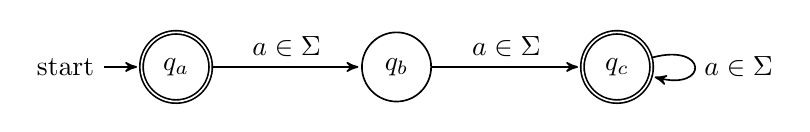
\begin{tikzpicture}[->,>=stealth',shorten >=1pt,auto,node distance=2.8cm,
                    semithick]

  \node[accepting,initial,state] (A)              {$q_a$};
  \node[state]                   (B) [right of=A] {$q_b$};
  \node[accepting,state]         (C) [right of=B] {$q_c$};

  \path (A) edge              node {$a \in \Sigma$} (B)
        (B) edge              node {$a \in \Sigma$} (C)
        (C) edge [loop right] node {$a \in \Sigma$} (C);
\end{tikzpicture}
\end{document}